\subsubsection{automated}

Automating the splitting of the entire computation is appealing. Ideally, the whole process shoule be similar to the following figure:

\begin{figure}[ht] 
    \centering  
    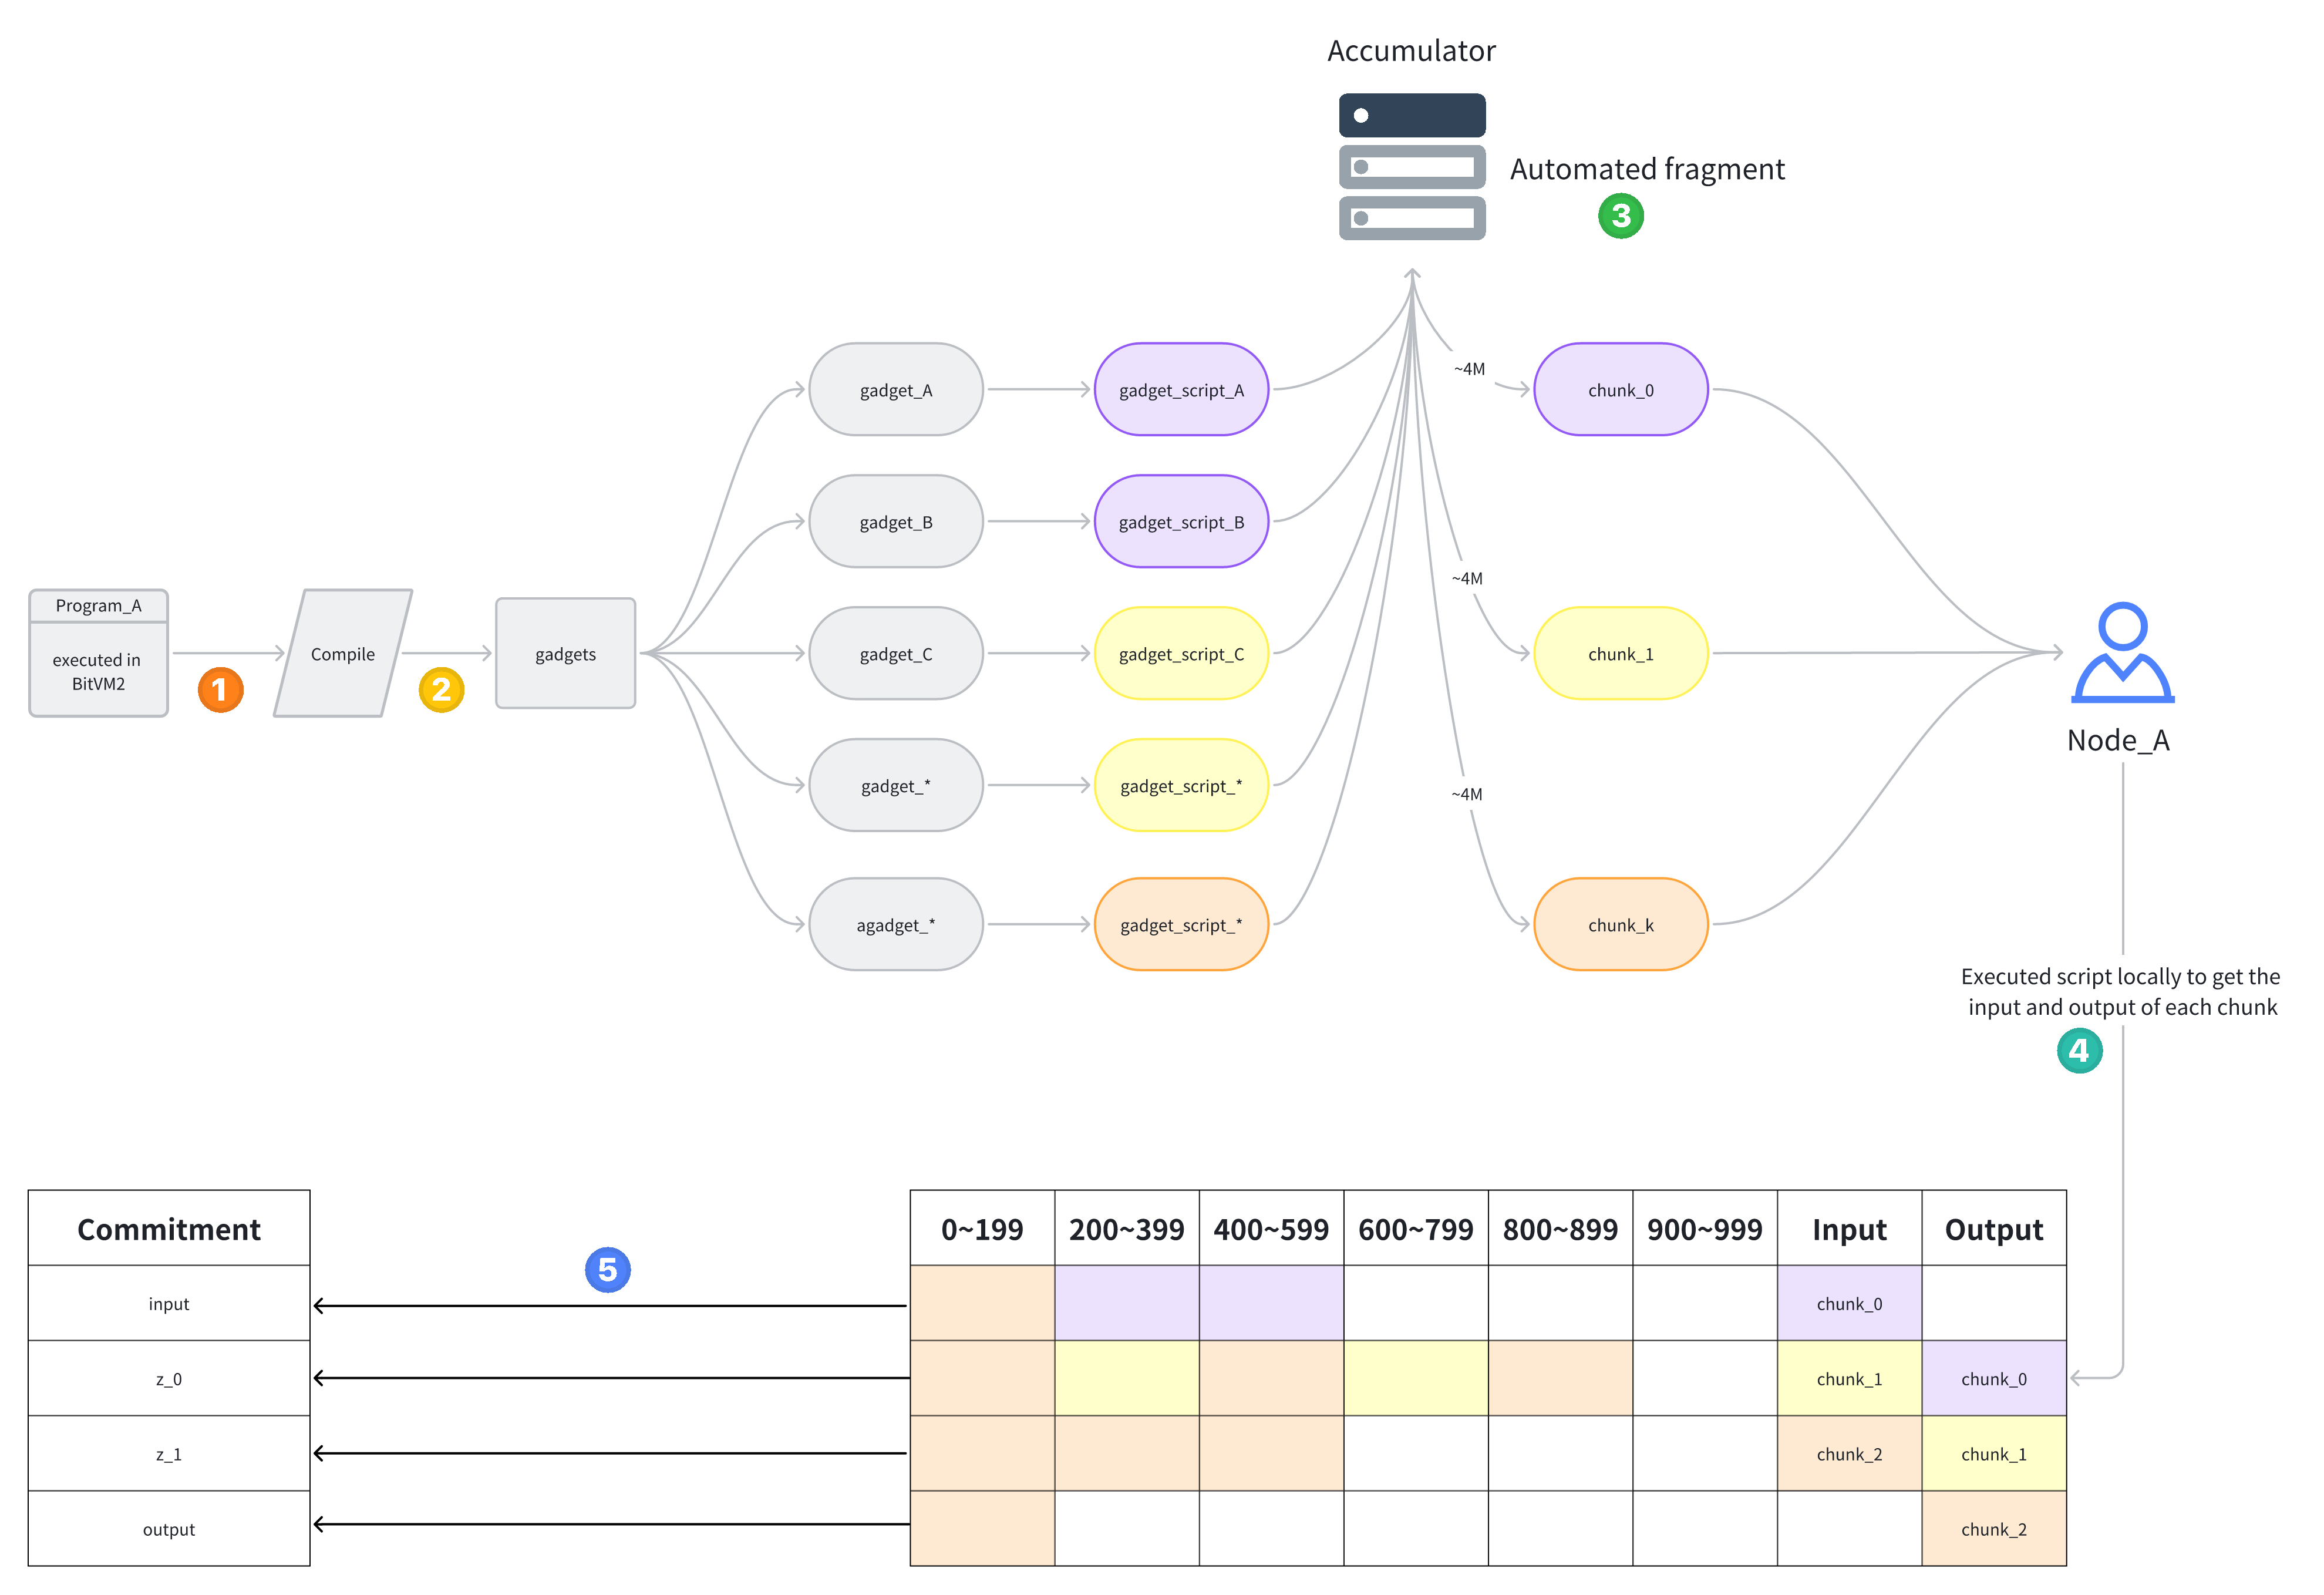
\includegraphics[width=0.85\columnwidth]{images/automated-fragment.png} 
    \caption{automated fragment}
    \label{fig:automated-fragment}
\end{figure}

The overall flow shoule be as follows:
\begin{itemize}
    \item The program will be complied into a set of customized gadgets first;
    \item Each gadget will correspond with a script gadget;
    \item The accmulator will begin to split all gadgets;
    \item Becasue each script gadget has a fixed size, these gadgets will be spilt as one chunk when their accumulated size is almost equal to 4M;
    \item Node A executes the script program locally to generate input and output for each chunk;
    \item All the input and output locate in stack, so Node A has to commit all the value in the stack;
\end{itemize}

It is important to note that stack depth is another factor that should be considered. In the automated approach, there are several constraints:
\begin{itemize}
    \item It is easy to exceed the stack depth limitation;
    \item It commits many values which will not be used in the current chunk;
    \item It must implememnt enough gadgets to support any computation, which means achieving turing completeness;
    \item Executing a large scirpt program is much slower;
    \item It increases the costs when verifying the expected input and output on-chain;
    \item The logic of each chunk is unreadable;
\end{itemize}

However, automated fragmentation has its advantages as well, such as generating the minimal number of script chunks. 
But since we do not upload all chunks to the Bitcoin network, the number of chunks is less of a concern unless their size becomes excessively large.
